\documentclass{beamer}
\mode<presentation>
{
  \usetheme{Luebeck}
  \usecolortheme{beaver}
  \usefonttheme{default}
  \setbeamertemplate{navigation symbols}{}
  \setbeamertemplate{caption}[numbered]
  \setbeamertemplate{theorems}[numbered]% Number theorem-related structures
}
\usepackage{hyperref}
\usepackage{tikz}
\usepackage{graphicx}
\usetikzlibrary{shapes,arrows}
\usepackage{natbib}
% include.tex

% \newcommand{\expit}[1]{\text{expit} #1}
% \newcommand{\logit}[1]{\text{logit} #1}

\def \R {{\mathbb{R}}}
\def \vbeta {{\boldsymbol \beta}}
\def \vnu {{\bf \nu}}
\def \vy {{\bf y}}
\def \vx {{\bf x}}
\def \vu {{\bf u}}
\def \vr {{\bf r}}
\def \vp {{\bf p}}
\def\vectorfontone{\bf}
\def\vone{{\bf 1}}
\def\vzero{{\bf 0}}
\def \vmu {{\boldsymbol \mu}}
\def \vnu {{\bf \nu}}
\def \vmuqbeta {{\vmu_{q(\vbeta)}}}
\def \vmubeta {{\vmu_{\vbeta}}}
\def \Sigmaqbeta {{\Sigma_{q(\vbeta)}}}
\def \Sigmabeta {{\Sigma_{\vbeta}}}
\def \va {{\bf a}}
\def \vtheta {{\bf \theta}}
\def \mX {{\bf X}}
\def \mZ {{\bf Z}}
\def \mR {{\bf R}}
\def \mC {{\bf C}}
\def \mI {{\bf I}}
\def \mLambda {{\boldsymbol \Lambda}}
\def \mSigma {{\boldsymbol \Sigma}}
\def \B {{\text{B}}}

\def\ds{{\displaystyle}}

\def\diag{{\mbox{diag}}}
\def\bbE{\mathbb{E}}

\title{Why is my code so slow?}
\author{Mark Greenaway}

%\begin{frame}
%Abstract

%Why is my code so slow?

%Many of us have been frustrated by running a program to perform a numerical
%experiment or a calculation and having it take a long time. In this talk, I
%will give a brief history of computers as it relates to performance, touching
%on cache hierarchy, the end of Moore's Law, multicore/GPUs and distributed
%computing. I will explain the latencies within a modern computer system, and
%the implications of this. I'll briefly provide a methodology for measuring and
%optimising the speed of programs.  Finally, I'll provide a glimpse into the
%future of computing and why it's going to be better than the present/past.

%This talk is supposed to be accessible to everyone, and as such, there will be
%no assumed knowledge.

%Mark Greenaway did a PhD supervised by A/Prof John Ormerod in computational
%statistics. He enjoys High Performance Computing, programming in statically
%typed languages, drinking too much coffee and listening to heavy metal music.
%Preferably all at the same time.
%\end{frame}

\begin{document}

\begin{frame}
	\maketitle
\end{frame}

\begin{frame}{Who am I?}
	\begin{itemize}
		\item Mark Greenaway, kind of old
		\item Bachelor of Computer Science, UWS, 1995--1997
		\item I have a UNIX/Linux upbringing, having used Linux since 1993
		% \item Over a decade of software engineering experience. I now lead a small team at the Commonwealth Bank, working on microservices for security
		\item Data Scientist at Commonwealth Bank
		\item
			\begin{itemize}
				\item Bachelor of Pure Mathematics and Statistics (Honours I), USyd, 2006--2009
				\item Masters of Biostatistics
				\item PhD in Computational Statistics (accepted with minor revisions), working with A/Prof John Ormerod
			\end{itemize}
	\end{itemize}
	I'm very opinionated, but I will attempt to present facts and let you decide for yourselves. If you want to know my opinion, read my Twitter at @certifiedwaif or ask me
\end{frame}

\begin{frame}{Why do mathematicians or statisticians care about computers at all?}
	\begin{itemize}
		\item I'm a computational statistician, so that informs my perspective
		\item The Bayesian perspective: Bayes' Theorem
			$$p(\vtheta|\vy, \mX) \propto \int p(\vy|\vtheta, \mX) p(\vtheta) d \vtheta$$ \\
			Many of the resulting integrals are analytically intractable and must be evaluated numerically
			\note{Bayesians know how to solve any statistical estimation problem, by turning your model specification into an integral we can't do}
		\item Relieves us of computational burden - we can't do many problems of practical interest with paper and pen
		\item{Numerical Recipes} -- All numerical problems seem to break down to function evaluation or linear algebra. If you're an applied mathematician, maybe differential equation solvers as well? 
	\end{itemize}
\end{frame}

\begin{frame}{Why does the speed of your code matter?}
	\begin{itemize}
		\item If your programs complete in seconds, or minutes, maybe they're fast enough
	already.  If they start to take minutes or hours, maybe not
	\note{and you're waiting for the
	results before you can do anything else, the speed of your code dictates the
	speed of your work/research.  For some areas of research, like computational fluid
dynamics, bioinformatics or others, computational speed becomes the limiting factor}

		\item Time is money, and $\text{speed} \propto \text{time}^{-1}$. So speed is money.

		\item An order of magnitude isn't just more of the same.  New things become possible
			\note{for example, the difference between powering a land vehicle and being able to get and keep it airborne is about a factor of ten New things become possible when you have access to this much computing power -- different approaches. Bigger problems, more dimensions, $p >> n$}
		\item \emph{Example: Bayesian Model Averaging} -- The amount of computation is extreme, and runtimes of days, weeks or months are not unheard of. It has been unfavorably compared to cryptocurrency mining \note{which contributes to climate change CO_2}

		\item If a primary output of your research is software, then you're likely to be
			judged on how quickly that software runs
			\note{In my field, every paper includes
			both numerical results and runtimes. If you can produce an equally numerically
			accurate result in less runtime, your software is better and you can publish a
		paper on that.}

		\item If you're writing software for other people to use, and it takes too long to run, they just won't use it
	\note{I worked as an applied statistician for years. If a model took more than a few minutes to run, I'd usually just give up and try something else. The reason I ended up back here is that I ran a model which took ten minutes to run and then failed to converge (!). This \emph{really} pissed me off.}
	\end{itemize}
\end{frame}

\begin{frame}{Caveat: When does the speed of your code \emph{not} matter?}
	\begin{itemize}

		\item Speed can mean different things in different contexts. Maybe what
		matters isn't how fast the computer runs your code, but how quickly you
		can do your analysis and move on to something else.
		\texttt{R}/\texttt{tidyverse} and \texttt{python}/\texttt{pandas}
		optimises for this
		
		\item What really matters is the speed of your research \note{Is your
		thesis finished yet? Have you written that paper? How's that grant
		coming along?} \note{You need to balance the amount of time spent on
		getting software to run faster against the amount of time actually saved
		by having it run for less time.}
		
		\item Optimising code to run faster should not trump every other
		research goal
		
		\item Maybe your time is better spent writing a paper or a grant, making
		a plot look better, or working on a thesis chapter? It's your call
		
	\end{itemize}
\end{frame}

\begin{frame}{Is it worth the time?}
	As with most things, there's an xkcd comic which is relevant.

	\begin{figure}
		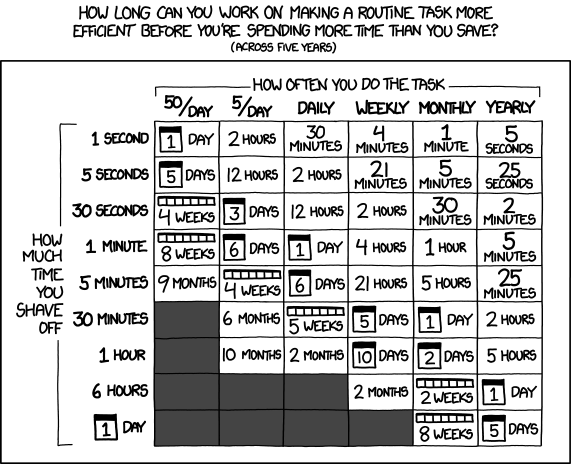
\includegraphics[scale=0.25]{is_it_worth_the_time.png}
	\end{figure}

	Making code faster isn't an end in itself. You can easily spend more time
	than you save. And programmer time is worth \emph{a lot} more than computer
	time.
\end{frame}

\begin{frame}{What do computers actually do? - CPU}
	A computer consists of a few major components.
	\begin{itemize}
		\item The Central Processing Unit (CPU) does a few things
			\begin{enumerate}
				\item arithmetic/logic
				\item conditional and unconditional branching
				\item reading/writing memory
				\item input/output to devices like keyboards, display adapters, disks, network interfaces, \ldots
		\end{enumerate}

		They do this by running very simple instructions, like \texttt{mov
		\%eax, 10} which moves the value $10$ into the \texttt{eax} register on
		an Intel CPU.
		
		\item A CPU runs an instruction in between one and a few clock cycles,
		but it runs \emph{billions} of these instructions per second. This gives
		the illusion of intelligence
		
	\end{itemize}
\end{frame}

\begin{frame}{What do computers actually do? -- Memory}
	\begin{itemize}
		\item CPUs have built in memory locations, called registers. The CPU's
		instructions can operate on these, or on memory on some architectures.
		Because the registers are on the chip, they're super fast
		
		\item For working with more data than can fit in the registers, we use
		memory off the CPU called RAM to load and store our data. It's cheaper,
		but slower to read and write
		
		\item That memory only lasts as long as the computer is on, so we load
		and save our data more permanently on disks. Those are cheaper and
		bigger, but slower still
		
		\item Computers can also communicate with each other over a network.
			\\
			If you're communicating between computers that
			are close together e.g. in the same rack or data centre, this is not too slow.
			But if they're far apart (say, California
			and the Netherlands) then this can be \emph{very} slow\note{. We're limited by
			the speed of light}
	\end{itemize}
\end{frame}

\begin{frame}{Memory hierarchy}
	\begin{itemize}
		\item This introduces the concept of a \emph{memory hierarchy}
		\item Some memory is very fast e.g. registers, but extremely expensive,
		so we don't have much of it to work with
		\item Some memory is very cheap, but slow e.g. hard disks
		\item The fast and slow parts of our computers work together to get our
		work done in a reasonable time, without costing too much
		\item You can think of a computer as a network of interconnected components,
		communicating with each other
		\item This communication takes \emph{time}!
		\item Understanding and working within this limitation is the key to
		making your code run faster
	\end{itemize}
\end{frame}

% Diagram: https://stackoverflow.com/questions/28815848/does-each-core-has-its-own-private-set-of-registers
\begin{frame}{A diagram of a CPU -- Intel core i7 Nehalem microarchitecture}
	\begin{figure}
		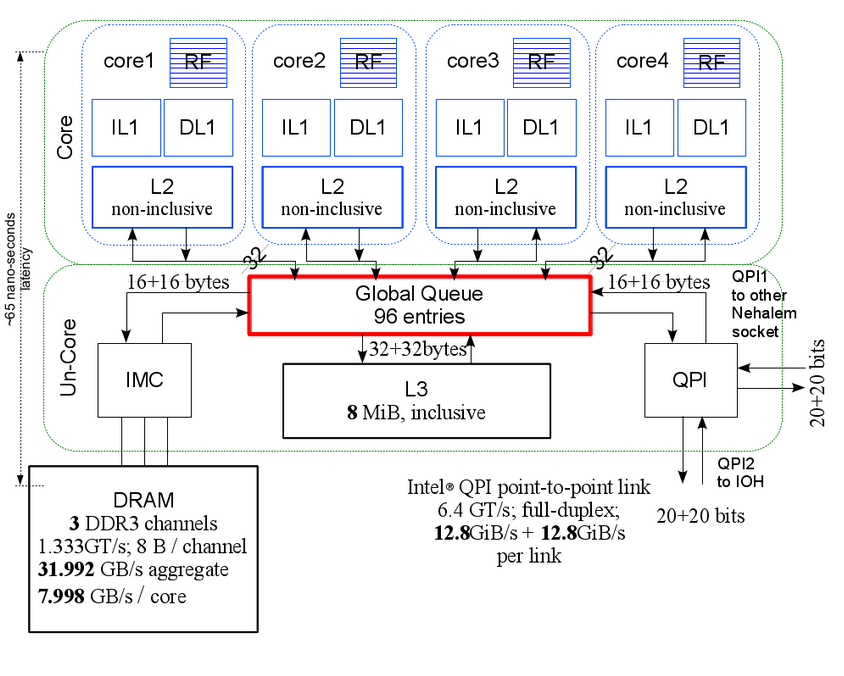
\includegraphics[scale=0.5]{Intel_core_i7.png}
	\end{figure}
\end{frame}

\begin{frame}{What do computers actually do? -- Software}
	We need to tell our computers what to do
	\begin{itemize}
		\item The Operating System kernel manages computer resources like scheduling when
			user programs run, which memory each program uses and how to access to the hardware to
			read the keyboard or display something on the monitor
		\item User level programs ask the kernel to do things for
			them, like allocate memory, start a process, read a file or send data over the
			network to another computer
       \item User level programs can also do things like read and write their
	   own memory or do logic and arithmetic
	\end{itemize}
\end{frame}

\begin{frame}{Programming languages}
	We tell our computers what to do using programming languages
	\begin{itemize}	

		\item Computers run assembly language. Computers were originally
		programmed in assembly or machine code, but this took a long time, and
		was tedious and error prone\note{show an example, the dot\_product}
		
		\item To allow programmers to be more productive, higher level languages
		like Fortran and C were invented

		\item  And then even more high level ones, like R and Python. Python and R are
		``glue'' languages that make calling C and Fortran easy, should you need to

		\item There are two major ways that code gets converted to instructions for computers to run: \emph{compilers} and \emph{interpreters}
			\begin{itemize}
				\item{compiler} -- Convert an entire program into assembly language at once
				\item{interpreter} -- Interpret a statement into assembly language, then execute it
			\end{itemize}
	\end{itemize}
\end{frame}

\begin{frame}{Differences between programming languages}
	\begin{itemize}	
		\item C and Fortran require you to manually allocate and deallocate
		memory, and declare types. No type inference yet
		\note{Unsafe memory access, leading to the
		possibility of segmentation faults where you attempt to access a piece
		of memory that's not yours. You need to tell them what type your
		variables are so it knows how much memory they need, and how that memory
		is laid out}
		
		\item R and Python use reference-counting garbage collection to manage
		memory for you, and are safe and dynamically typed.
		\\
		They're also
		interpreted -- you can interact with them using a REPL (Read-Eval-Print-Loop).
		% \note{They manage the
		% layout and allocation/deallocation of memory for you}. \\
		\\
		They are much easier to learn, and way more productive for most people.
		These languages have come to dominate Data Science
	\end{itemize} 
\end{frame}

\begin{frame}{Higher level languages are more productive, but nothing comes for free}
	\begin{itemize}
		\item There is a substantial difference in speed - 10 times to 100 times
		is typical

		\item R and Python get around this by implementing their array operations
		very efficiently in C or Fortran, and by being able to call functions written
		in C or Fortran very easily

		\item This is why people say ``\texttt{for} loops are slow''
		-- it's a half-truth

		\item \texttt{for} loops are slow in R or Python.
		But \texttt{for} loops in C or Fortran are the fastest kind of
		loop you can write \footnote{on a single core -- more on this later} -- indeed, the loop your CPU was \emph{designed}
		to execute

		\note{BLAS executes your for loops for you in highly optimised Fortran
		or C, where they're fast}
		
	\end{itemize}
\end{frame}

\begin{frame}{A brief history of computer hardware -- 1970s}
	\begin{itemize}
		\item 8-bit, clock speeds measure in kilohertz, in the 8-bit 6502 era
		memory was fast enough to keep up with the CPU.
		\item Most of the programming
		languages that we use today use a flat memory model which dates from this time,
		and assume that all memory takes the same amount of time to access i.e. that there
		is no memory hierarchy
		\item This has
		not been true since at least 1985 for most of us
		\item Moore's Law is in full flight, and CPU clock speeds are roughly doubling every year
	\end{itemize}
\end{frame}

\begin{frame}{A brief history of computer hardware -- 1980s to 2006}
	\begin{itemize}
		\item For a while, Moore's Law continues unabated --
		Every year, the clock speed doubles.
		This exponential increase goes on for some time, from ~1 MHz (Commodore 64) to
		~5.2 GHz (i9-12900K, 24 threads, 30 MB L3 cache, 76.8 GB/s memory bandwidth). Good times!!!
		% https://ark.intel.com/content/www/us/en/ark/products/134599/intel-core-i912900k-processor-30m-cache-up-to-5-20-ghz.html

		\item	Clock speeds keep increasing, but memory and disk speed does \emph{not} keep pace.
		Hard disks can read 10Mb/s to 20Mb/s (~10,000 times slower than memory!) \\
	\emph{Solution:} Cache/Memory hierarchy! RAID disk arrays!
	\end{itemize}
\end{frame}

\begin{frame}{A brief history of computer hardware -- 2006 to the present day}
	\begin{itemize}
		\item	2006 to now -- As time goes on, physical limits begin to be reached, and progress grinds to a halt.
		\item You can buy a 5.2 GHz CPU now, but are we at the end of Moore's Law? \textbf{YES!} (\cite{SophieWilson})\\
			\note{About 2006, clock speeds stopped increasing.}
			\emph{Solutions:} Vector units! More cores! GPUs! Distributed computing! \footnote{To a point, but we'll talk about that later too}
		\item Solid State Drives become available, which are much faster than hard disks,
			able to transfer 550 MB/s (nearly approx 2 orders of magnitude faster!!! Only 140 times slower than memory). % Only 140 times slower than RAM.
		\item So why can't we go any faster? It's expensive to make things any smaller (billions of dollars)
		\item And then you have to dissipate the heat \ldots
	\end{itemize}
	
\end{frame}

% TODO: Show the graph
% https://github.com/karlrupp/microprocessor-trend-data
% https://community.cadence.com/cadence_blogs_8/b/breakfast-bytes/posts/sophie2
\begin{frame}{The end of Moore's Law -- a graph}
	\begin{figure}
		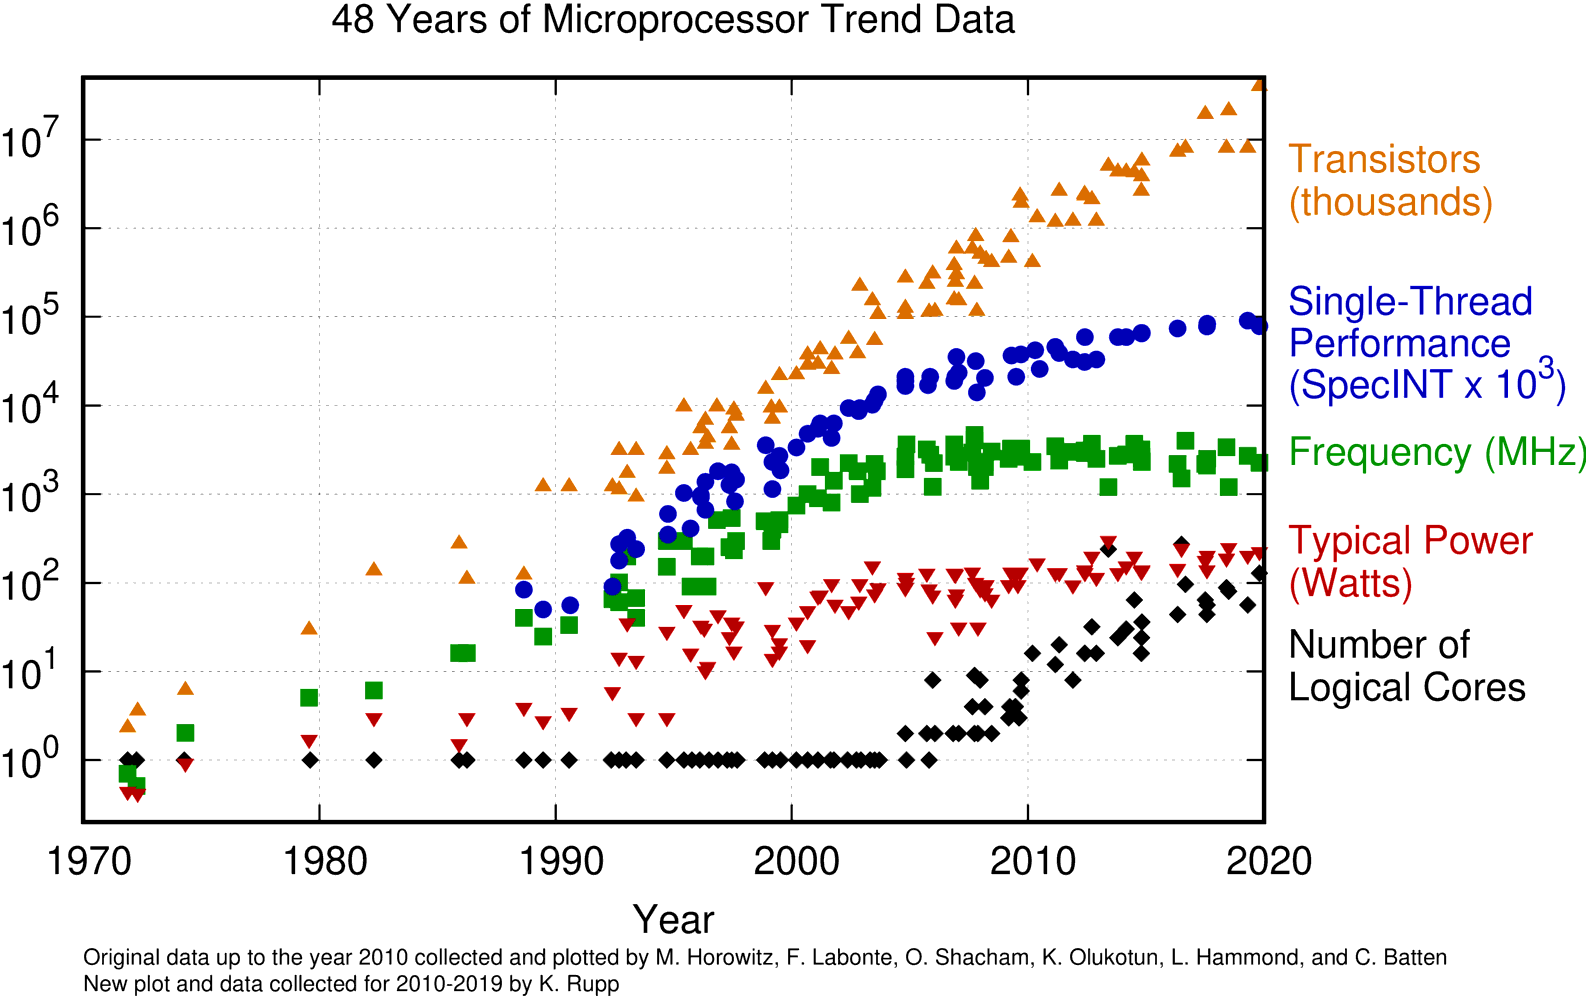
\includegraphics[scale=0.2]{48-years-processor-trend.png}
	\end{figure}
\end{frame}

\begin{frame}{Heat, and the end of Moore's Law}
	\begin{itemize}
	\item As you run your processor faster and faster, it generates more and more heat, in a
	very small space. This heat is really difficult to dissipate. If you run your
	CPU any faster, it can fail or melt.

	\item One of the ways that CPUs deal with this is by decreasing their clock
	frequency temporarily and spinning their fans until the heat goes away, then
	increasing the clock frequency again.
	
	\item Another way is by turning parts of the chip off. Obviously, you can't use
	those parts when they're off.

	\item These things all rob your CPU of the speed you thought you were paying
	for.  The Intel CPU in my work-issued 2018 MacBook Pro frequently runs hot enough to boil
	an egg.
	
	\end{itemize}
\end{frame}

\begin{frame}{Power density}
	\begin{figure}
		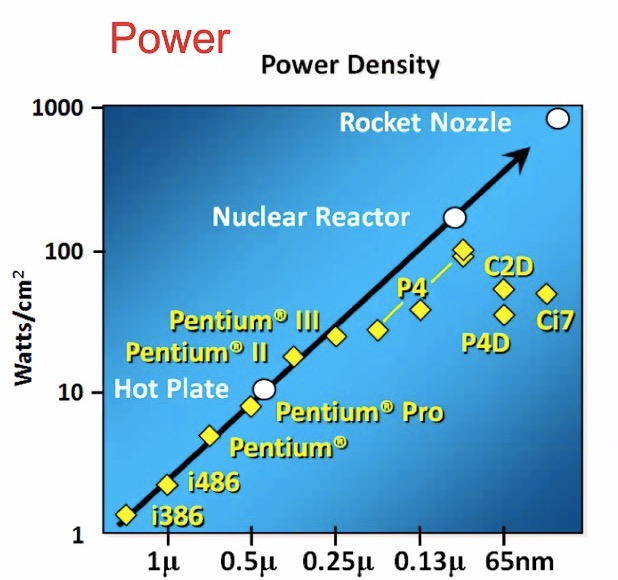
\includegraphics[scale=0.3]{Power_Density.jpg}
	\end{figure}
\end{frame}

% Credit: https://gist.github.com/jboner/2841832
\begin{frame}{How long things take on a computer}
	Everything you do on a computer takes time. Some things are fast, and some of them are
	comparatively very slow. How fast something is is dictated by how far from the CPU
	it is
	{
	\tiny
			\begin{tabular}{lllll}
				Task & ns & us & ms & Note \\
				\hline
				L1 cache reference                &          0.5 ns &&& \\
				Branch mispredict                 &          5   ns &&& \\
				L2 cache reference                &          7   ns &&                   &14x L1 cache \\
				Mutex lock/unlock                 &         25   ns &&& \\
				Main memory reference             &        100   ns &&                   &20x L2 cache, 200x L1 cache \\
				Compress 1K bytes with Zippy      &      3,000   ns &      3 us&& \\
				Send 1K bytes over 1 Gbps network &     10,000   ns &     10 us&& \\
				Read 4K randomly from SSD*        &    150,000   ns &    150 us&         &~1GB/sec SSD \\
				Read 1 MB sequentially from memory&    250,000   ns &    250 us&& \\
				Round trip within same datacenter &    500,000   ns &    500 us&& \\
				Read 1 MB sequentially from SSD*  &  1,000,000   ns &  1,000 us  & 1 ms &~1GB/sec SSD, 4X memory \\
				Disk seek                         & 10,000,000   ns & 10,000 us  &10 ms &20x datacenter roundtrip \\
				Read 1 MB sequentially from disk  & 20,000,000   ns & 20,000 us  &20 ms &80x memory, 20X SSD \\
				Send packet CA to the Netherlands and back again & 150,000,000 ns & 150,000 us & 150 ms \\
				\hline
			\end{tabular}
		}
			What you should focus on here aren't the specific \emph{numbers}, but the difference in
	\emph{magnitude}. Don't feel bad if you didn't know -- some of this is highly counter-intuitive
\end{frame}

% Credit: https://twitter.com/DynamicWebPaige/status/1044443943679668224/photo/1
\begin{frame}{Latency -- graphically}
	\begin{figure}
		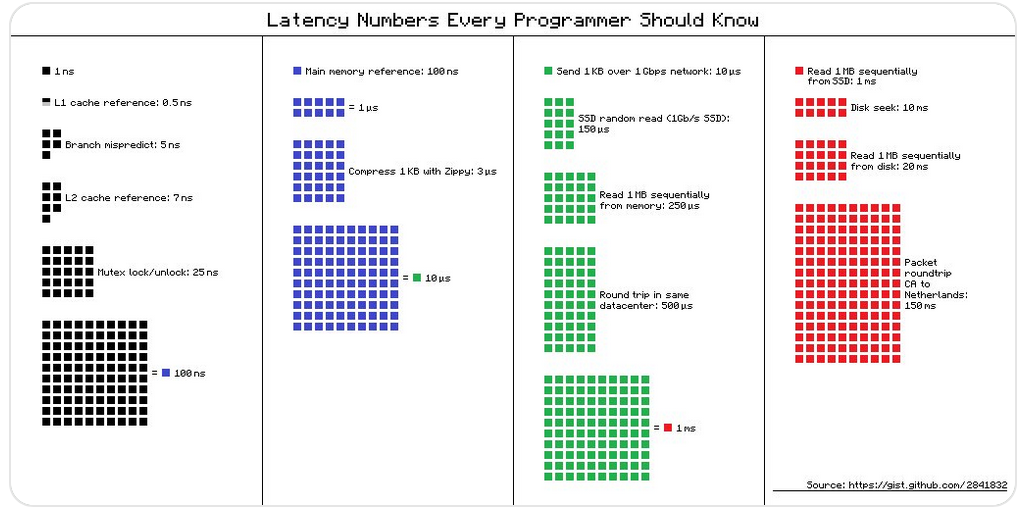
\includegraphics[scale=0.60]{Latency_graphically.png}
	\end{figure}
\end{frame}

% Credit: Page 573, Fluent Python
\begin{frame}{In human terms}
	The difference in magnitude is so great that it can be hard to conceptualise.
	Let's try to put it in human terms.

	\begin{tabular}{lll}
		Device & CPU cycles & Proportional human timescale \\
		\hline
		Register & 1 & 1 second \\
		L1 cache & 3 & 3 seconds \\
		L2 cache & 14 & 14 seconds \\
		RAM & 250 & 4 minutes \\
		Network access within the data centre & 10,000 & $2 \frac{2}{3}$ hours \\
		Disk & 41,000,000 & 1.3 years \\
		Network access over the Internet & 240,000,000 & 7.6 years \\
		\hline
	\end{tabular}
\end{frame}

\begin{frame}{A metaphor}
	\begin{itemize}
	\item Getting something from a register or cache is like grabbing it from right
	in front of you
	\item Getting something from RAM is like taking the elevator
	from Level 5 of the Foundry to the ground floor.

	\item Getting something from the network within the same data centre is like
	travelling from Central to Penrith and back by train
	
	\item Getting something from disk is like walking 2,400 km, from Sydney to
	Melbourne and back, or from Sydney to New Zealand, if you could walk on
	water
	
	\item Getting something from the network over the Internet is like walking halfway around the Earth,
	on foot. \note{If you walked from Sydney to China, then kept going through Russia,
	kept right on and starting crossing the Arctic ice till you got to the North
	Pole, and pressed on till you made it to Iceland.} Which you kind of did,
	but at a fraction of the speed of light
	\end{itemize}
\end{frame}

\begin{frame}{What should we do to speed things up?}

	\begin{quote}
		Premature optimisation is the root of all evil -- Donald Knuth
	\end{quote}
		
	Take a disciplined approach

	\begin{itemize}

		\item Make sure your program is correct first, and that you have
		automated or at least repeatable tests

		\item Have your program in version control
		
		\item Measure where the time is spent with a line profiler. Don't guess! \emph{Measure}!
		You will guess \emph{wrong}
		
		\item Change from a higher strength operation to a lower strength
		operation that does the same thing where the bottleneck is.

		\item For example,
		in R, change a \texttt{for} loop to a vector operation, or use a lower
		level language
		
		\item Check correctness and measure the performance again. If your
		program is faster, congratulations, you're winning!
		
		\item If not, back out the change and try again
		
		\item Repeat until your program is fast enough
	\end{itemize}

\end{frame}

\begin{frame}{Parallel Programming}
	\begin{itemize}
		\item You can't buy a single core computer any more, so you should at least be
		aware of multithreaded programming, parallelism and concurrency

		\item Processes and Threads -- your operating system presents two major
		abstractions for programs to run in, threads and processes
		
		\item Cores have their own registers and L1 and L2 caches. L3 cache is
		shared amongst all cores. Memory and memory bandwidth is also shared
		
		\item Threads within a process have shared memory whereas processes each
		have their own memory
		
		\item Different libraries use either threads or processes. For example,
		OpenMP is shared memory concurrency while
		\texttt{mclapply}/\texttt{future} is multi-process
	\end{itemize}		
\end{frame}

\begin{frame}{Shared memory concurrency is \emph{hard}! Distributed programming is \emph{hard}!}
	\begin{itemize}
		\item Shared memory concurrency is notoriously difficult!
		\item It opens up the possibility of \emph{race conditions}
		\item Code that does not have any race conditions is said to be \emph{thread-safe}
		\item For most of us, it's better to use a simpler programming model that
		places some restrictions on what we can do, but gives us a better chance
		of getting our parallel and concurrent programs right
		\begin{itemize}
			\item Map/Reduce
			\item Spark
			\item Futures in Python or R
			\item \texttt{furrr}/\texttt{mclapply}
			\item Rust's concurrency model
		\end{itemize} 
	\end{itemize}
\end{frame}	

\begin{frame}{Parallel Programming -- continued}
	\begin{itemize}
		\item Languages which use reference-counting garbage collection are a
		textbook example of a race condition. They are not even \emph{remotely}
		thread-safe -- examples are R and Python
		\item This is the dreaded Global
		Interpreter Lock (GIL) which has proven fiendishly difficult to remove,
		although there is some good news on that front
		\item Python programs have difficulty taking advantage of multiple threads,
		item and hence multiple CPU cores
		\item The same problem exists
		in R, and will be even more difficult to remove, if it ever is
	\end{itemize} 
\end{frame}

\begin{frame}{Parallel and Concurrent Programming -- Asynchronous I/O}
	\begin{itemize}
		\item \emph{However}, Python is really good at asynchronous I/O. You
		should take full advantage of this, especially over the network
		\item Python has had multi-threading since before 1.0.0, and has language
		features to make asynchronous code easier.
		\item The
		\texttt{concurrent.future} module is really good.
		\item \texttt{asyncio} is also really good
		\item R has something similiar, with the \texttt{future} package.
	\end{itemize}
\end{frame}

\begin{frame}{Parallel programming for Linux/Mac OS X and Windows}
	\begin{itemize}

		\item Linux and Mac OS X use very similiar UNIX kernels -- System V and
		BSD respectively. Programmers greatly prefer this
		
		\item Windows uses its own kernel, developed entirely by Microsoft

		\item Windows and UNIX have different operating system kernels, with
		different APIs. Windows presents a different threading API than UNIX
		
		\item \texttt{R} for Windows is a port of a UNIX program to Windows, but
		it is not a complete port.
		
		\item R for Windows is using the UNIX threading and multiprocess APIs
		through a compatibility library provided by a port of \texttt{gcc} to
		Windows, to try to make Windows look like UNIX to R.  But it doesn't
		work very well, which is why parallel programming in R doesn't work well
		on Windows \note{In fact, R for Windows doesn't work very well. Just ask
		the R for Windows maintainer, Jeroen Ooms @opencpu.  He'll quite happily
		tell you this}
		
	\end{itemize}
\end{frame}

\begin{frame}{Python and R have really good libraries}
	\begin{itemize}
		\item Python is the most popular language in the world, and the majority
		of Data Scientists use it
		\item As such, enormous engineering effort has been and will continue to 
		be put into making it faster and better
		\item Great examples of good libraries include \texttt{numpy}, or
		\texttt{TensorFlow}
		\item \texttt{TensorFlow} works by having the programmer specify a computational
		graph in Python, then optimising this entire graph so that it can run
		in parallel on CPUs and/or GPUs
		\item \texttt{PySpark} translates your Python code into equivalent
		Java/Scala code, which is then optimised and run on the JVM
		\item \texttt{RStan} does something similiar, where you specify your model
		in a modelling language, and then it is translated to C++, compiled and
		run
	\end{itemize}
\end{frame}

\begin{frame}{Amdahl's Law: Quick derivation}
	Every program has a parallelisable part, and a non-parallelisable part.
	The run-time on a single core is
	$$
	P + (1 - P)
	$$
	If we have $n$ cores, we can split the parallel apart up between them. then
	the run-time drops to
	$$
	\frac{P}{n} + (1-P)
	$$
	but the serial part takes the same amount of time to run.
	
	$\text{Speed} \propto \text{1/time}$, so the speed-up you can get by adding
	more cores is
	$$
	\frac{1}{\frac{P}{n} + (1-P)}
	$$

	This is a function of both the number of cores $n$ and the parallel fraction
	of your code $P$. As $n \to \infty$ this tends to $\frac{1}{1-P}$, so the
	runtime of your program becomes dominated by the serial part.
\end{frame}

\begin{frame}{Consequences of Amdahl's Law}
	\begin{figure}
		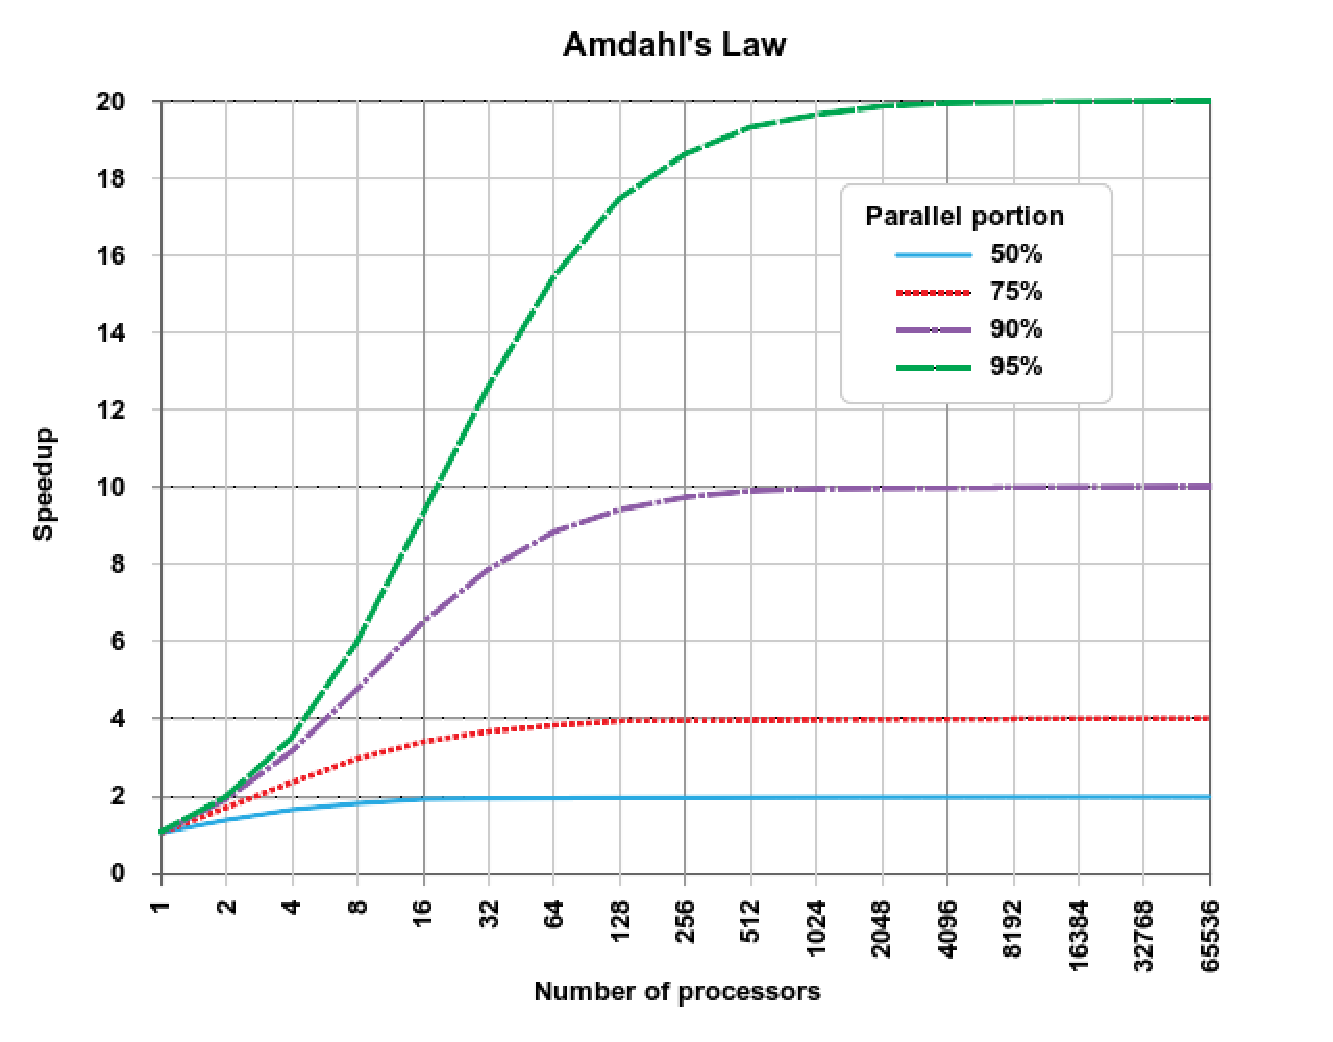
\includegraphics[scale=0.45]{AmdahlsLaw.pdf}	
	\end{figure}
\end{frame}

\begin{frame}{Consequences of Amdahl's Law -- continued}
	\begin{itemize}
		\item The good news for us as data scientists is that the kinds of computational
	problems we solve are typically embarassingly parallel (P=0.95 or even higher). \\
		\item The bad news is that this still only helps so much. We face a Law of Diminishing
		Returns as we continue to add more cores, spending exponentially more money
		on computational hardware for ever poorer returns. Even if you had infinite
		cores, you can still only speed up your code by 20 times! \\
		\item For other types of program, the news is even worse! Compilers are perhaps
		P=0.75, and web browsers are between P=0.5 and P=0.75.
		\item This law is just as applicable to distributed storage
		as it is to processors
	\end{itemize}
\end{frame}

\begin{frame}{Example -- Summing numbers}

	{\small
	Why do we need a serial part in a parallel program? Let's say we're adding up $n$ numbers, and we have $n$ processors.
	}
	\begin{figure}
		\scalebox{0.25}{\input{example.tex}}
		\caption{Summing $n$ numbers on $n$ processors}
	\end{figure}
	{\small
	We can get the partial sums on $n/2$ of the processors, but then we have to
	keep combining them to get our final answer. This takes at least as many steps
	as the depth of the tree -- $\log_2{(n)}$. 

	If we're adding up $8$ numbers, we still need to do at least $3$ sets of operations,
	even though we have $8$ processors! And for the majority of the time, most of the
	processors are unable to do anything to help.
	}
\end{frame}

\begin{frame}{Amdahl's Law applies to any parallel task}
	\begin{itemize}
	\item This doesn't just apply to processors. It applies to any kind of task we're
	trying to speed up by sub-dividing it among multiple resources	

	\item Imagine that you were sorting a large data set. You can divide the data set
	up among $n$ computers and sort the subsets individually. But you do have to
	merge and combine them to get the final sorted data set

	\item The graph of computation is exactly the same as for the example of summing
	numbers above. You have to combine your partial answers to get your final answer

	\item The graph of computation dictates how fast a task can ever be made to
	run, no matter how much hardware you have

	\end{itemize}
\end{frame}

\begin{frame}{What's coming? -- Better hardware -- higher core counts, GPUs with more cores}
	\begin{itemize}
		\item We have a large Spark cluster with hundreds of nodes, and over a thousand cores. We should leverage that
		\item Intel is releasing CPUs with higher core counts
		\item NVidia is releasing GPUs with more and more cores
		\item Faster SSDs and networking. Faster memory buses, Unified Memory Architecture (UMA)
		\item 
		\begin{itemize}
			\item Intel's 40 year dominance of the processor market may finally
				be ending.
			\item Apple, Google, Amazon, Microsoft and others are
					designing and releasing their own custom ARM processors.
			\item Performance is \emph{finally} meeting or exceeding that of
					comparable Intel processors, with less power usage and cost.
					It's about time we saw some real competition in this space!

		\end{itemize}
	\end{itemize}
\end{frame}

\begin{frame}{What's coming -- Better languages -- allowing you to use this hardware more easily}
	\begin{itemize}
		\item The languages we typically use are quite old! C and R date from
		the 70s, and Python was release in 1991
		\item Computers have changed a lot since then, and there's been enormous progress in Programming
		Language Theory in that time
		\item Just-In-Time compilers/interpilers, type inference
			\begin{itemize}
				\item Julia
				\item Kotlin
				\item Rust (fearless concurrency)
			\end{itemize} 
        \item Type inference and interpilers mean that statically typed languages,
			  are now more usable for some of the tasks that we routinely do
		\item Better libraries e.g. TensorFlow, Spark
		\item Better compilers
	\end{itemize}
\end{frame}

\begin{frame}{But Moore's Law really is over}
	\begin{itemize}
		\item Any increases in computational speed are going to come from higher thread
		counts, better memory buses, GPUs or distributed computing

		\item There is nothing else on the horizon, because physical limits are being
		reached. If we ran our CPUs any faster, \emph{they'd melt} (\cite{SophieWilson})

		\item Quantum computing will not save us, because quantum computers are only
		good at what quantum computers are good at. Great if you're factoring large
		composite numbers to break people's encryption, rather less good if you're
		trying to fit models with \texttt{xgboost}

		\item
		\begin{quote}
			People will have to adjust their expectations -- Sophie Wilson
		\end{quote}
	\end{itemize}
\end{frame}

\begin{frame}{What should I do?}
	\begin{itemize}
		\item Measure performance systematically. Don't guess, use a profiler
		
		\item Take advantage of the memory hierarchy

		\item Keeping your data set small can yield huge performance benefits
		if you can stay higher up the memory hierarchy for a greater proportion
		of the time

		\item The fastest kind of communication is no communcation. If you can
		structure your parallel computations so that they don't have to talk, they'll
		be faster

		\item If you can, get your data into RAM, and keep it there! This is exactly what
		Spark does

		\item Distributed programming has become \emph{way} easier. Learn to program
		clusters e.g. Spark

		\item Do your disk and network I/O concurrently. If you're going to walk
		from Sydney to Iceland, at least take all of your walks at the same time!
		Don't do them one after the other!

		% \item I assembled a small HPC cluster for \$100 per node. Ask me how! Computers
		% have become very cheap. People will often give you their computer from 2006,
		% failing to realise that because of the end of Moore's Law, it's still state of the
		% art
	\end{itemize}
\end{frame}

\begin{frame}{What should I do -- continued}
	\begin{itemize}
		\item If you're doing all of your computing on your laptop, you're \emph{really}
		missing out. Laptops are trying to minimise power consumption to increase battery life, and
		can't effectively dissipate heat, so they're down-clocking most of the time.
		You should at least know how to use servers

		\item The cloud is someone else's computer, and they'll rent by the
		hour. Or the second. Computing is now a commodity. You can rent a pretty
		good server (AWS Graviton2 c6g.16xlarge, EC2 Spot) for \$0.60 an hour on
		AWS. \note{Use one all day for less than you probably paid for lunch!}

		\item Learn to program or leverage GPUs or heterogeneous processors if you can
		
	\end{itemize}
\end{frame}

\begin{frame}{References}
\bibliographystyle{authordate1}
\bibliography{whyismycodesoslow.bib}
\end{frame}
\end{document}